\documentclass[12pt]{article}    
\usepackage{ucs} 
\usepackage[utf8x]{inputenc}
\usepackage[russian]{babel}  
\usepackage{float}
\usepackage{amsmath}
\title{Псевдоэксперимент №6}
\author{Хафизов Фанис}
\usepackage[pdftex]{graphicx}
\usepackage{multirow}
\begin{document}
	\begin{figure}
		\centering
		
\includegraphics[width=0.3\linewidth]{logo}
	\end{figure}
	\maketitle
	\newpage
	\section{Определение коэффициентов зависимости}
	Предположение Тейлора:
	$$R=t^\alpha E^\beta \rho^\gamma$$
	$[R] = 1$ м\\
	$[t] = 1$ с\\
	$[E] = 1$ кг$\cdot$м$^2/$с$^2$\\
	$[\rho] = 1$ кг/м$^3$\\
	Из метода размерностей получим систему уравнений:
	\begin{equation*}
		\begin{cases}
			1=2\beta-3\gamma\\
			0=\beta+\gamma\\
			0=\alpha-2\beta
		\end{cases}
	\end{equation*}
	\begin{equation*}	
		\begin{cases}
			\alpha = \frac{2}{5}\\
			\beta = \frac{1}{5}\\
			\gamma = -\frac{1}{5}
		\end{cases}
	\end{equation*}
	$$R = t^\frac{2}{5}E^\frac{1}{5}\rho^{-\frac{1}{5}}$$
	\section{Оценка выделившейся энергии}
	Для каждой точки посчитаем $t^\frac{2}{5}$, чтобы зависимость $R(t^\frac{2}{5})$ была линейна.
	\begin{table}[H]
		\begin{tabular}{|l|l|l|l|}
			\hline
			№ & t, с & R, км & $t^\frac{2}{5}$, с$^\frac{2}{5}$ \\ \hline
			1 & 4    & 0,55  & 1,74                             \\ \hline
			2 & 8    & 0,70  & 2,30                             \\ \hline
			3 & 16   & 0,95  & 3,03                             \\ \hline
			4 & 28   & 1,25  & 3,79                             \\ \hline
			5 & 46   & 1,50  & 4,62                             \\ \hline
		\end{tabular}
	\end{table}
	Построим график зависимости $R(t^\frac{2}{5})$.
	\begin{figure}[H]
		\centering
		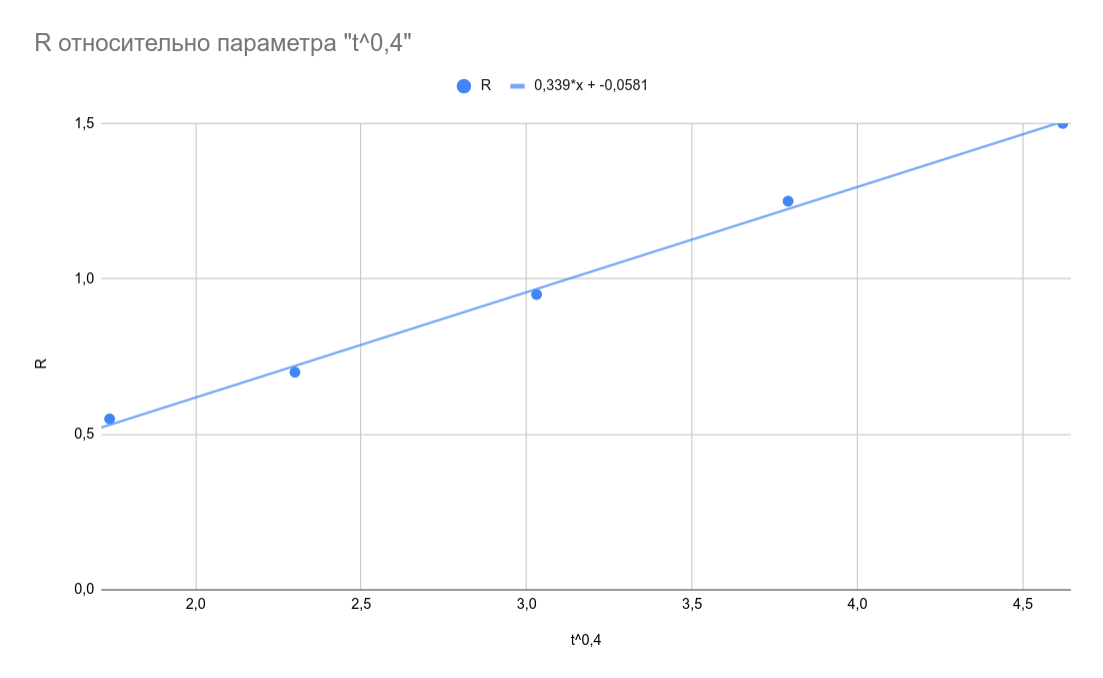
\includegraphics[width=\linewidth]{graph}
		\caption{График зависимости $R(t^\frac{2}{5})$}
	\end{figure}
	Угловой коэффициент наклона равен $k = 0,339\cdot10^3$ м/с$^{0,4}$. С другой стороны, он также равен $E^{0,2}\rho^{-0,2}$.\\
	$E = \rho\cdot k^5 = 1,3\cdot10^3\cdot33,9^5=5,82\cdot10^{10}$ Дж $=58,2$ ГДж
	\section{Ответ}
	$E=58,2$ ГДж
\end{document}